% blog-title: Probability, Filtrations, and Adaptive Data
% blog-date: 2026-06-18
% blog-description: The probability grammar behind bandit proofs: filtrations, conditional expectation, martingale differences, adaptive confidence intervals, and post-selection bias.
% blog-lang: en

\documentclass[en,nofont,11pt]{elegantbook}

\title{Probability, Filtrations, and Adaptive Data}
\subtitle{The Hidden Grammar of Bandit Proofs}
\author{Tang}
\institute{Tang's Machine Learning Blog}
\date{2026-06-18}
\version{1.0.0}
\bioinfo{Topic}{Probability, Filtrations, Adaptive Data, Bandit Proofs}
\cover{assets/blog-cover.jpg}

\usepackage{fontspec}
\ifdefined\setCJKmainfont
\else
  \usepackage[UTF8,scheme=plain,fontset=none]{ctex}
\fi
\usepackage{xcolor}
\usepackage{listings}
\usepackage{float}
\usepackage{tcolorbox}
\tcbuselibrary{breakable, listings, skins}
\usetikzlibrary{arrows.meta,positioning,calc,decorations.pathmorphing,decorations.pathreplacing,fit,backgrounds,patterns,shapes.geometric}

\IfFontExistsTF{Microsoft YaHei}{
  \setCJKmainfont{Microsoft YaHei}
  \setCJKsansfont{Microsoft YaHei}
  \setCJKmonofont{Microsoft YaHei UI}
}{
  \IfFontExistsTF{Noto Serif CJK SC}{
    \setCJKmainfont{Noto Serif CJK SC}
    \setCJKsansfont{Noto Sans CJK SC}
    \setCJKmonofont{Noto Sans Mono CJK SC}
  }{}
}

\definecolor{blogAccent}{HTML}{1F6F8B}
\definecolor{blogInk}{HTML}{172026}
\definecolor{blogCodeBg}{HTML}{F5F7F8}
\definecolor{blogCodeBorder}{HTML}{D6E2E8}
\definecolor{blogKeyword}{HTML}{B23A48}
\definecolor{blogString}{HTML}{287D4F}
\definecolor{blogComment}{HTML}{687783}

\lstdefinestyle{blogcode}{
  basicstyle=\ttfamily\small,
  keywordstyle=\bfseries\color{blogKeyword},
  stringstyle=\color{blogString},
  commentstyle=\itshape\color{blogComment},
  numberstyle=\scriptsize\color{blogComment},
  numbers=left,
  numbersep=8pt,
  showstringspaces=false,
  breaklines=true,
  tabsize=2,
  columns=fullflexible,
  keepspaces=true
}

\newtcblisting{codeblock}[2][]{
  listing only,
  breakable,
  enhanced,
  colback=blogCodeBg,
  colframe=blogCodeBorder,
  arc=2mm,
  boxrule=0.4pt,
  left=6mm,
  right=2mm,
  top=1mm,
  bottom=1mm,
  listing options={style=blogcode, language=#2},
  #1
}

\hypersetup{
  colorlinks=true,
  linkcolor=blogAccent,
  urlcolor=blogAccent,
  citecolor=blogAccent
}

\addbibresource{tex/bandits-references.bib}

\definecolor{filtrationBlue}{RGB}{27,63,119}
\definecolor{filtrationLightBlue}{RGB}{235,243,253}
\definecolor{filtrationSoftBlue}{RGB}{224,237,250}
\definecolor{filtrationBrown}{RGB}{130,68,18}
\definecolor{filtrationLightBrown}{RGB}{255,248,235}
\colorlet{deepblue}{filtrationBlue}
\colorlet{lightblue}{filtrationLightBlue}
\colorlet{softblue}{filtrationSoftBlue}
\colorlet{deepbrown}{filtrationBrown}
\colorlet{lightbrown}{filtrationLightBrown}

\newtcolorbox{keyidea}[1][]{
  enhanced,breakable,
  colback=lightblue,colframe=deepblue,
  boxrule=0.8pt,arc=2mm,
  title=Key idea,#1
}

\newtcolorbox{thinkbox}[1][]{
  enhanced,breakable,
  colback=lightbrown,colframe=deepbrown,
  boxrule=0.8pt,arc=2mm,
  title=Think,#1
}

\newtcolorbox{plainbox}[1][]{
  enhanced,breakable,
  colback=white,colframe=black!35,
  boxrule=0.5pt,arc=1mm,#1
}

\newcommand{\E}{\mathbb{E}}
\newcommand{\Pp}{\mathbb{P}}
\newcommand{\F}{\mathcal{F}}
\newcommand{\one}{\mathbf{1}}
\newcommand{\R}{\mathbb{R}}
\newcommand{\given}{\,\middle|\,}
\newcommand{\argmax}{\operatorname*{arg\,max}}

\begin{document}
\maketitle
\frontmatter
\tableofcontents
\mainmatter

\chapter{The real problem: data is not waiting on a table}

In supervised learning, the data set usually arrives first.  We open the file, see rows of examples, and then fit a model.  The model may be complicated, but the data has already been collected.

Bandit learning reverses the order.  The algorithm acts first.  The data appears because of the action.

That one reversal is the source of almost all probability in bandit theory.

\begin{center}
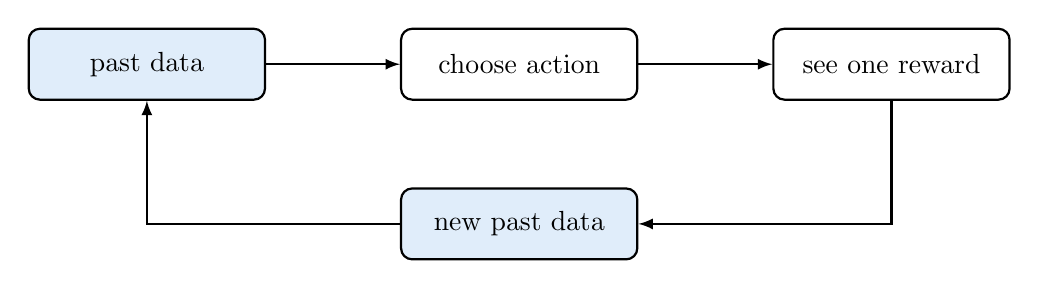
\begin{tikzpicture}[node distance=1.7cm,>=latex,thick]
\node[draw,rounded corners,fill=softblue,minimum width=3.0cm,minimum height=0.9cm] (past) {past data};
\node[draw,rounded corners,fill=white,minimum width=3.0cm,minimum height=0.9cm,right=of past] (action) {choose action};
\node[draw,rounded corners,fill=white,minimum width=3.0cm,minimum height=0.9cm,right=of action] (reward) {see one reward};
\node[draw,rounded corners,fill=softblue,minimum width=3.0cm,minimum height=0.9cm,below=1.1cm of action] (newpast) {new past data};
\draw[->] (past) -- (action);
\draw[->] (action) -- (reward);
\draw[->] (reward) |- (newpast);
\draw[->] (newpast) -| (past);
\end{tikzpicture}
\end{center}

The hard part is not that rewards are random.  The hard part is that the learner chooses which randomness it will see.  A bad early choice can starve an arm of data.  A lucky early reward can make a bad arm look good.  A confidence interval that is valid at one fixed time can become misleading if we keep peeking and stop when it looks favorable.

This note is about the grammar that prevents those mistakes.

\begin{keyidea}
A bandit proof does not start with ``let $\Omega$ be a probability space.''  It starts with a simple rule of order:
\[
\text{past} \quad \longrightarrow \quad \text{action} \quad \longrightarrow \quad \text{reward}.
\]
The formal probability notation is just a clean way to respect this order.
\end{keyidea}

\chapter{Random variables: numbers before they are seen}

A random variable is a number whose value has not yet been revealed.

For a Bernoulli reward, the number is either $0$ or $1$.  If the click probability is $p$, then
\[
X=\begin{cases}
1, & \text{with probability }p,\\
0, & \text{with probability }1-p.
\end{cases}
\]

The expectation is the long-run average value.  Here there are only two possible values, so the calculation is direct:
\begin{align}
\E[X]
&= 1\cdot \Pp(X=1) + 0\cdot \Pp(X=0) \\
&= 1\cdot p + 0\cdot (1-p) \\
&= p. \label{eq:bernoulli_mean}
\end{align}

If we observe $n$ independent rewards $X_1,\ldots,X_n$, the sample average is
\[
\widehat p_n = \frac{1}{n}\sum_{s=1}^n X_s.
\]

The sample average is random before the experiment is run.  Its expectation is easy to compute:
\begin{align}
\E[\widehat p_n]
&= \E\left[\frac{1}{n}\sum_{s=1}^n X_s\right] \\
&= \frac{1}{n}\sum_{s=1}^n \E[X_s] \\
&= \frac{1}{n}\sum_{s=1}^n p \\
&= p. \label{eq:sample_mean_unbiased}
\end{align}

This is the first comfort: the sample average points to the right target on average.

But an average can point in the right direction and still wobble.  Probability inequalities measure the wobble.

\chapter{Error bars: turning randomness into a usable statement}

For Bernoulli rewards, Hoeffding's inequality says
\begin{equation}
\Pp\left(\left|\widehat p_n-p\right|\geq \varepsilon\right)
\leq 2\exp(-2n\varepsilon^2). \label{eq:hoeffding}
\end{equation}

This formula is not meant to be memorized as decoration.  It answers a practical question: how large should the error bar be if we want failure probability at most $\delta$?

Start from the right-hand side and set it equal to $\delta$:
\begin{align}
2\exp(-2n\varepsilon^2) &= \delta,\\
\exp(-2n\varepsilon^2) &= \frac{\delta}{2},\\
-2n\varepsilon^2 &= \log\left(\frac{\delta}{2}\right),\\
2n\varepsilon^2 &= \log\left(\frac{2}{\delta}\right),\\
\varepsilon^2 &= \frac{\log(2/\delta)}{2n},\\
\varepsilon &= \sqrt{\frac{\log(2/\delta)}{2n}}. \label{eq:hoeffding_radius}
\end{align}

So we may write the fixed-time confidence statement as
\begin{equation}
\Pp\left(
\left|\widehat p_n-p\right|
\leq
\sqrt{\frac{\log(2/\delta)}{2n}}
\right)
\geq 1-\delta. \label{eq:fixed_time_ci}
\end{equation}

\begin{thinkbox}
The phrase ``fixed time'' is doing real work.  The statement above is about one sample size $n$ chosen before looking at the data.  It is not automatically a promise that the same error bar works after repeatedly looking at the data and stopping at a convenient time.
\end{thinkbox}

\chapter{A first warning: peeking changes the game}

Suppose a coin is fair, so $p=1/2$.  If we toss it exactly $200$ times and look once at the end, a standard error bar behaves roughly as expected.

But if we look after every toss and stop the moment the running average looks high, the final number is no longer an ordinary fixed-time average.  We have selected a time because the noise looked favorable.

This is not a philosophical issue.  It appears directly in simulation.

\begin{figure}[H]
\centering

\includegraphics[width=0.82\linewidth]{assets/filtrations/figures/fixed_vs_stopped_means.pdf}
\caption{The fixed-time mean is centered near the true value $0.5$.  The adaptively stopped mean is shifted upward because we stop when the noise is favorable.}
\label{fig:fixed_vs_stopped}
\end{figure}

The same idea appears when we keep checking an error bar many times.

\begin{figure}[H]
\centering

\includegraphics[width=0.82\linewidth]{assets/filtrations/figures/false_alarm_comparison.pdf}
\caption{A normal-looking error bar is reasonable for one final look, but repeated peeking with the same bar creates many false alarms.  A union-bound bar is crude but safe.}
\label{fig:false_alarm}
\end{figure}

The experiment used $20{,}000$ runs of a fair Bernoulli process with horizon $T=200$.  The stopped rule begins checking after $20$ samples and stops when the running mean first exceeds $0.56$.

\begin{table}[H]
\centering
\small
\begin{tabular}{lr}
\toprule
Quantity & Value \\
\midrule
True Bernoulli mean & 0.500 \\
Probability of stopping early & 0.555 \\
Average fixed-time mean & 0.500 \\
Average stopped mean & 0.548 \\
One final look false alarm with normal bar & 0.057 \\
Many peeks false alarm with same normal bar & 0.414 \\
Many peeks false alarm with union bar & 0.000 \\
Post-selection average of one fixed arm & 0.500 \\
Post-selection average of empirical winner among 20 arms & 0.705 \\
\bottomrule
\end{tabular}
\caption{The important number is not the exact decimal.  The important lesson is that adapting to the observed noise changes the distribution of what we report.}
\label{tab:simulation_results}
\end{table}

\chapter{Histories: the learner's notebook}

In a bandit problem, the learner accumulates a notebook.

At the beginning of round $t$, the notebook contains all past actions and rewards:
\begin{equation}
H_{t-1}=(A_1,R_1,A_2,R_2,\ldots,A_{t-1},R_{t-1}).
\end{equation}

Then the learner chooses an action using only this notebook:
\begin{equation}
A_t = \pi_t(H_{t-1}).
\end{equation}

Then the environment reveals one reward:
\begin{equation}
R_t \sim \text{reward distribution of arm }A_t.
\end{equation}

Then the notebook becomes
\begin{equation}
H_t=(H_{t-1},A_t,R_t).
\end{equation}

A filtration is just the mathematical name for this growing notebook.  We write
\begin{equation}
\F_t = \text{all information contained in }H_t.
\end{equation}

So $\F_{t-1}$ means ``everything known before choosing and observing at time $t$.''

\begin{keyidea}
A filtration is not a mysterious object.  It is the learner's notebook, ordered by time.  The only rule is that the algorithm may read old pages before acting, but it cannot read the next reward before choosing the next action.
\end{keyidea}

\chapter{Conditional expectation: averaging after the past is known}

The ordinary expectation $\E[X]$ averages before anything is known.  The conditional expectation $\E[X\mid \F_{t-1}]$ averages after the past notebook has been opened.

For a bandit reward, suppose arm $i$ has mean $\mu_i$.  If the learner chooses $A_t=i$, then
\begin{equation}
\E[R_t \mid \F_{t-1}, A_t=i] = \mu_i.
\end{equation}

But $A_t$ itself is chosen using $\F_{t-1}$, so once the past is known, $A_t$ is also known.  Hence
\begin{equation}
\E[R_t \mid \F_{t-1}] = \mu_{A_t}. \label{eq:conditional_reward_mean}
\end{equation}

Now define the one-step noise
\begin{equation}
\eta_t = R_t - \mu_{A_t}.
\end{equation}

Using \eqref{eq:conditional_reward_mean},
\begin{align}
\E[\eta_t\mid \F_{t-1}]
&= \E[R_t-\mu_{A_t}\mid \F_{t-1}] \\
&= \E[R_t\mid \F_{t-1}] - \mu_{A_t} \\
&= \mu_{A_t} - \mu_{A_t} \\
&= 0. \label{eq:martingale_difference}
\end{align}

This tiny equation is everywhere in bandit theory.  It says: after we condition on the past, the remaining reward noise is fair.

\chapter{Martingale differences: fair noise after conditioning}

A sequence $\eta_t$ satisfying
\begin{equation}
\E[\eta_t\mid \F_{t-1}]=0
\end{equation}
is called a martingale difference sequence.

The name is less important than the picture.  At time $t$, the learner may be very clever.  It may choose $A_t$ using every previous reward.  But after the action is fixed, the new noise still has mean zero.

\begin{center}
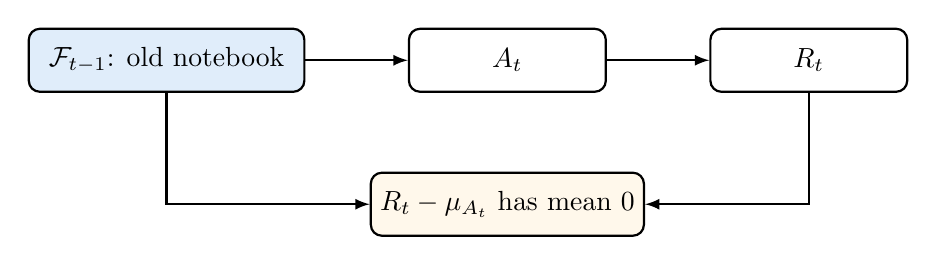
\begin{tikzpicture}[>=latex,thick,node distance=1.3cm]
\node[draw,rounded corners,fill=softblue,minimum width=3.5cm,minimum height=0.8cm] (F) {$\F_{t-1}$: old notebook};
\node[draw,rounded corners,fill=white,minimum width=2.5cm,minimum height=0.8cm,right=of F] (A) {$A_t$};
\node[draw,rounded corners,fill=white,minimum width=2.5cm,minimum height=0.8cm,right=of A] (R) {$R_t$};
\node[draw,rounded corners,fill=lightbrown,minimum width=3.3cm,minimum height=0.8cm,below=1.0cm of A] (noise) {$R_t-\mu_{A_t}$ has mean $0$};
\draw[->] (F) -- (A);
\draw[->] (A) -- (R);
\draw[->] (R) |- (noise);
\draw[->] (F) |- (noise);
\end{tikzpicture}
\end{center}

This is why adaptive data is not hopeless.  The actions are adaptive, but the reward noise remains conditionally centered.

\chapter{Adaptive sample means}

For arm $i$, define the number of times it has been pulled by time $t$:
\begin{equation}
N_i(t)=\sum_{s=1}^t \one\{A_s=i\}.
\end{equation}

Define the empirical mean of arm $i$:
\begin{equation}
\widehat\mu_i(t)=
\frac{\sum_{s=1}^t \one\{A_s=i\}R_s}{N_i(t)}
\quad\text{when }N_i(t)>0.
\end{equation}

The numerator has two pieces:
\begin{align}
\sum_{s=1}^t \one\{A_s=i\}R_s
&= \sum_{s=1}^t \one\{A_s=i\}(\mu_i + R_s-\mu_i) \\
&= \mu_i\sum_{s=1}^t \one\{A_s=i\}
+ \sum_{s=1}^t \one\{A_s=i\}(R_s-\mu_i) \\
&= \mu_i N_i(t)
+ \sum_{s=1}^t \one\{A_s=i\}(R_s-\mu_i).
\end{align}

Divide by $N_i(t)$:
\begin{align}
\widehat\mu_i(t)-\mu_i
&=
\frac{1}{N_i(t)}
\sum_{s=1}^t \one\{A_s=i\}(R_s-\mu_i). \label{eq:adaptive_empirical_error}
\end{align}

The error is still an average of centered noise terms, but the number of terms is random and chosen adaptively.  That is the reason for filtrations and anytime confidence bounds.

The key centering step is
\begin{align}
\E\left[\one\{A_s=i\}(R_s-\mu_i)\mid \F_{s-1}\right]
&= \one\{A_s=i\}\,\E\left[(R_s-\mu_i)\mid \F_{s-1},A_s=i\right] \\
&= \one\{A_s=i\}\cdot 0 \\
&= 0. \label{eq:adaptive_centering}
\end{align}

The indicator $\one\{A_s=i\}$ is allowed because the action is chosen from the past.  It is known at the moment we average over the new reward.

\begin{thinkbox}
This is the essence of adaptive data: the learner can choose which arm to sample, but it cannot choose the new random fluctuation after the arm has been chosen.  That remaining fluctuation is still fair after conditioning on the past.
\end{thinkbox}

\chapter{The union bound: a simple way to be right many times}

The union bound says that the probability that at least one bad event happens is at most the sum of the probabilities of the bad events.

For events $E_1,\ldots,E_m$,
\begin{equation}
\Pp\left(\bigcup_{j=1}^m E_j\right)\leq \sum_{j=1}^m \Pp(E_j). \label{eq:union_bound}
\end{equation}

A one-line proof uses indicators.  For every outcome,
\begin{equation}
\one\left\{\bigcup_{j=1}^m E_j\right\}
\leq
\sum_{j=1}^m \one\{E_j\}.
\end{equation}

Take expectations:
\begin{align}
\Pp\left(\bigcup_{j=1}^m E_j\right)
&= \E\left[\one\left\{\bigcup_{j=1}^m E_j\right\}\right] \\
&\leq \E\left[\sum_{j=1}^m \one\{E_j\}\right] \\
&= \sum_{j=1}^m \E[\one\{E_j\}] \\
&= \sum_{j=1}^m \Pp(E_j).
\end{align}

Now suppose we want confidence intervals for $K$ arms and $T$ possible times.  There are at most $KT$ things we want to be simultaneously correct about.

Give each one failure probability
\begin{equation}
\delta' = \frac{\delta}{KT}.
\end{equation}

For each arm-time pair, Hoeffding gives
\begin{equation}
\Pp\left(
|\widehat\mu_i(t)-\mu_i|>
\sqrt{\frac{\log(2/\delta')}{2N_i(t)}}
\right)
\leq \delta'.
\end{equation}

Substitute $\delta'=\delta/(KT)$:
\begin{align}
\sqrt{\frac{\log(2/\delta')}{2N_i(t)}}
&= \sqrt{\frac{\log(2KT/\delta)}{2N_i(t)}}. \label{eq:union_radius}
\end{align}

Then the union bound says that all these intervals are correct together with probability at least $1-\delta$.

This is crude.  Modern analyses often use sharper time-uniform tools.  But the union-bound version is the first clean proof pattern, and it already explains why logarithms appear in bandit regret bounds.

\chapter{From probability to UCB}

UCB is built from one sentence:

\begin{quote}
Choose the arm whose plausible optimistic value is largest.
\end{quote}

At time $t$, define the radius
\begin{equation}
\operatorname{rad}_i(t)
=\sqrt{\frac{\log(2KT/\delta)}{2N_i(t)}}.
\end{equation}

The optimistic index is
\begin{equation}
\operatorname{UCB}_i(t)
=\widehat\mu_i(t)+\operatorname{rad}_i(t).
\end{equation}

The algorithm chooses
\begin{equation}
A_{t+1}\in \argmax_i \operatorname{UCB}_i(t).
\end{equation}

The confidence event is
\begin{equation}
\mathcal{G}=
\left\{
\forall i,\forall t:\ |
\widehat\mu_i(t)-\mu_i|
\leq \operatorname{rad}_i(t)
\right\}. \label{eq:good_event}
\end{equation}

On $\mathcal{G}$, every empirical mean is close to its truth at every relevant time.  That single event drives the UCB proof.

\section{The pull-count argument, line by line}

Let $i^*$ be an optimal arm and let $i$ be a suboptimal arm.  Define the gap
\begin{equation}
\Delta_i=\mu_{i^*}-\mu_i>0.
\end{equation}

Suppose UCB pulls arm $i$ at some time.  Since UCB chose $i$ instead of $i^*$,
\begin{equation}
\widehat\mu_i + \operatorname{rad}_i
\geq
\widehat\mu_{i^*}+\operatorname{rad}_{i^*}. \label{eq:ucb_chose_i}
\end{equation}

On the good event $\mathcal{G}$,
\begin{equation}
\widehat\mu_{i^*}+\operatorname{rad}_{i^*}
\geq \mu_{i^*}. \label{eq:optimal_still_plausible}
\end{equation}

Combining \eqref{eq:ucb_chose_i} and \eqref{eq:optimal_still_plausible},
\begin{equation}
\widehat\mu_i + \operatorname{rad}_i
\geq \mu_{i^*}. \label{eq:chosen_index_above_opt}
\end{equation}

Again on $\mathcal{G}$,
\begin{equation}
\widehat\mu_i \leq \mu_i + \operatorname{rad}_i. \label{eq:suboptimal_upper}
\end{equation}

Substitute \eqref{eq:suboptimal_upper} into \eqref{eq:chosen_index_above_opt}:
\begin{align}
\mu_i + \operatorname{rad}_i + \operatorname{rad}_i
&\geq \mu_{i^*},\\
2\operatorname{rad}_i
&\geq \mu_{i^*}-\mu_i,\\
2\operatorname{rad}_i
&\geq \Delta_i,\\
\operatorname{rad}_i
&\geq \frac{\Delta_i}{2}. \label{eq:radius_large}
\end{align}

Now plug in the radius:
\begin{align}
\sqrt{\frac{\log(2KT/\delta)}{2N_i(t)}}
&\geq \frac{\Delta_i}{2},\\
\frac{\log(2KT/\delta)}{2N_i(t)}
&\geq \frac{\Delta_i^2}{4},\\
4\log(2KT/\delta)
&\geq 2N_i(t)\Delta_i^2,\\
N_i(t)
&\leq \frac{2\log(2KT/\delta)}{\Delta_i^2}. \label{eq:ucb_pull_count_simple}
\end{align}

Depending on the exact convention for the radius, constants change.  The message does not change: a bad arm can only be pulled many times if its uncertainty radius is still large.  Once it has been sampled enough, its upper confidence bound drops below the optimal arm's plausible value.

\begin{keyidea}
The UCB proof is not magic.  It is a bookkeeping argument:
\[
\text{bad arm chosen}
\Rightarrow
\text{its uncertainty must still be large}
\Rightarrow
\text{it has not been sampled too often}.
\]
\end{keyidea}

\chapter{Post-selection bias: the quiet enemy}

Another common mistake is to look at many random estimates and then trust the largest one as if it had been chosen in advance.

Imagine $20$ arms.  In this experiment they are all identical: every arm has true mean $0.5$.  We sample each arm $20$ times and select the one with the largest empirical mean.

The selected arm looks much better than $0.5$, not because it is truly better, but because it won a noise contest.

\begin{figure}[H]
\centering

\includegraphics[width=0.82\linewidth]{assets/filtrations/figures/post_selection_bias.pdf}
\caption{When all arms have the same true mean, the best empirical arm is still biased upward.  Selection turns noise into apparent signal.}
\label{fig:post_selection}
\end{figure}

This is why bandit algorithms need explicit exploration rules.  Greedy selection tends to chase the current winner.  Confidence-based and posterior-based algorithms try to remember that the current winner may be winning only because the data is thin.

\chapter{Code implementation}

The simulation is deliberately small.  It is not a benchmark.  It is a microscope.

The first part compares one fixed-time average with an adaptively stopped average.

\begin{codeblock}[title={Adaptive stopping experiment.}]{Python}
for r in range(cfg.runs):
    x = rng.binomial(1, cfg.p, size=cfg.fixed_n)
    s = np.cumsum(x)
    t = np.arange(1, cfg.fixed_n + 1)
    m = s / t

    fixed_means[r] = m[-1]

    normal_radius = 1.96 * np.sqrt(0.25 / t)
    union_r = union_radius(t, cfg.alpha, cfg.fixed_n)
    final_normal_false_alarm[r] = abs(m[-1] - cfg.p) > normal_radius[-1]
    anytime_normal_false_alarm[r] = np.any(np.abs(m - cfg.p) > normal_radius)
    anytime_union_false_alarm[r] = np.any(np.abs(m - cfg.p) > union_r)

    eligible = np.where((t >= cfg.stop_start) & (m >= cfg.threshold))[0]
    if eligible.size > 0:
        j = int(eligible[0])
        stopped_times[r] = j + 1
        stopped_means[r] = m[j]
        stopped_by_rule[r] = True
    else:
        stopped_times[r] = cfg.fixed_n
        stopped_means[r] = m[-1]
        stopped_by_rule[r] = False
\end{codeblock}

The second part shows post-selection bias.

\begin{codeblock}[title={Post-selection experiment.}]{Python}
# All arms have the same true mean.  Any winner is a winner only because of noise.
samples = rng.binomial(1, cfg.p, size=(cfg.runs, cfg.k_arms, cfg.n_per_arm))
means = samples.mean(axis=2)
selected = means.max(axis=1)
ordinary = means[:, 0]
\end{codeblock}

The full script is included in the appendix and in the accompanying simulation file.

\chapter{What this chapter prepares}

The next bandit algorithms will use the same grammar repeatedly.

For UCB, the key object is a confidence event that holds across arms and times.

For Thompson sampling, the key object is a posterior distribution updated by the same history $\F_t$.

For best-arm identification, the key object is a stopping time: a random time at which the algorithm decides it has enough evidence.

For batched bandits, the key object is restricted adaptivity: the notebook is updated only at batch boundaries.

So probability is not a decorative layer.  It is the language that keeps time, information, and evidence in the correct order.

\begin{keyidea}
The deepest lesson is simple: in bandits, data has a timestamp.  A proof is correct only if it respects what was known before the action and what was revealed after the action.
\end{keyidea}

\chapter*{Appendix A. Symbol Table}
\addcontentsline{toc}{chapter}{Appendix A. Symbol Table}

\begin{longtable}{>{\raggedright\arraybackslash}p{0.22\linewidth}p{0.70\linewidth}}
\toprule
Symbol & Meaning \\
\midrule
\endfirsthead
\toprule
Symbol & Meaning \\
\midrule
\endhead
$A_t$ & action chosen at round $t$ \\
$R_t$ & reward observed after choosing $A_t$ \\
$H_t$ & history or notebook after round $t$ \\
$\F_t$ & filtration: all information contained in $H_t$ \\
$\mu_i$ & true mean reward of arm $i$ \\
$N_i(t)$ & number of pulls of arm $i$ by time $t$ \\
$\widehat\mu_i(t)$ & empirical mean of arm $i$ by time $t$ \\
$\Delta_i$ & suboptimality gap $\mu_{i^*}-\mu_i$ \\
$\eta_t$ & centered reward noise $R_t-\mu_{A_t}$ \\
$\operatorname{rad}_i(t)$ & confidence radius for arm $i$ at time $t$ \\
$\mathcal{G}$ & good event on which all confidence intervals are simultaneously correct \\
\bottomrule
\end{longtable}

\chapter*{Appendix B. Core Formulas}
\addcontentsline{toc}{chapter}{Appendix B. Core Formulas}

\begin{align}
\E[X] &= \sum_x x\,\Pp(X=x),\\
\widehat p_n &= \frac{1}{n}\sum_{s=1}^n X_s,\\
\Pp\left(|\widehat p_n-p|\geq \varepsilon\right) &\leq 2\exp(-2n\varepsilon^2),\\
\varepsilon_n(\delta) &= \sqrt{\frac{\log(2/\delta)}{2n}},\\
H_t &= (A_1,R_1,\ldots,A_t,R_t),\\
\E[R_t\mid \F_{t-1}] &= \mu_{A_t},\\
\E[R_t-\mu_{A_t}\mid \F_{t-1}] &=0,\\
N_i(t)&=\sum_{s=1}^t \one\{A_s=i\},\\
\widehat\mu_i(t)-\mu_i
&=\frac{1}{N_i(t)}\sum_{s=1}^t \one\{A_s=i\}(R_s-\mu_i),\\
\Pp\left(\bigcup_j E_j\right)&\leq \sum_j \Pp(E_j),\\
\operatorname{UCB}_i(t)&=\widehat\mu_i(t)+\sqrt{\frac{\log(2KT/\delta)}{2N_i(t)}}.
\end{align}

\chapter*{Appendix C. Full Simulation Code}
\addcontentsline{toc}{chapter}{Appendix C. Full Simulation Code}

\lstinputlisting[style=blogcode,language=Python,caption={Full simulation code.}]{assets/filtrations/probability-filtrations-simulation.py}

\backmatter
\nocite{lattimore2020bandit,bubeck2012,auer2002,howard2020timeuniform}
\printbibliography[heading=bibintoc,title={References}]

\end{document}
